\chapter{First Chapter Title}
\label{chapter:firstChapterTitle}
\graphicspath{ {./chapter01/Fig} }

\begin{itquote}
Snappy quote to characterize chapter.
\end{itquote}

\lipsum[2-3]

\section*{Learning Objectives}
\noindent\rule{\linewidth}{1pt}
By the end of this chapter, the reader should:
\begin{itemize}
\item 	\lipsum[6]
\item 	\lipsum[5]
\end{itemize}

\section{The First With A Table}
\label{section:the-first-section}

\lipsum[7]
A reference to Table~\ref{table:thisIsTheFirstTable}
\lipsum[8]

\begin{table}[h]
\caption{This is an important table.}
\label{table:thisIsTheFirstTable}
\begin{tabular}{|l|c|c|c|c|}
\hline
\rowcolor{Gray}
 & & \multicolumn{3} {c|} {Alternatives} \\ \hhline{|~|~|-|-|-|}
\rowcolor{Gray}
 \multirow{-2}{*}{Selection Criteria} & \multirow{-2}{*}{Weights}  & Project 1 & Project 2 & Project 3 \\ \hline
A (Match to skills) & 0.52 & 0.40 & 0.20 & 0.40 \\  \hline
B (Technical Complexity) & 0.12 & 0.40 & 0.30 & 0.30 \\ \hline
C (Creativity) & 0.09 & 0.45 & 0.20 & 0.35 \\ \hline
D (Market potential) & 0.18 & 0.05 & 0.35 & 0.60 \\ \hline
E (Industry sponsorship) & 0.09 & 0.00 & 1.0 & 0.00 \\ \hline
Score & & 0.31 & 0.31 & 0.38 \\ \hline
\end{tabular}
\end{table}


\lipsum[9]
A reference to Figure~\ref{figure:dilbertCommunication}.
\lipsum[10]

\begin{figure}[h]
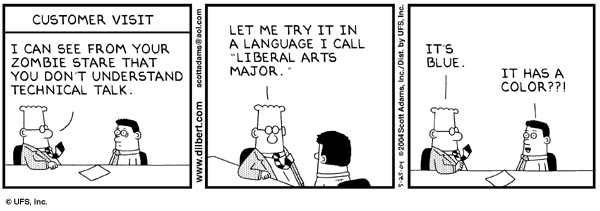
\includegraphics[width=5.5in,height=1.9in]{image1.png}
\caption{ The difficulties of communicating with the customer. (Dilbert © United Feature Syndicate. Reprinted by
permission.)}
\label{figure:dilbertCommunication}
\end{figure}


\lipsum[11]
A reference to Equation~\ref{equ:simpleEquation}.
\lipsum[12]


\begin{equation}
\label{equ:simpleEquation}
x = \int v(t) dt
\end{equation}

\lipsum[12]

\begin{example}{A Simple Example}
\label{example:aSimpleExample}
\emph{\textbf{\ul{Problem:}}} Consider.... \\	% Force line break for spacing
\noindent\emph{\textbf{\ul{Solution:}}} The parallel systems...
\end{example}

\lipsum[13]

\begin{itemize}
\item
  US Bureau of Labor Statistics, \url{http://stats.bls.gov}.
  different industry sectors.
\item
  US Government Official WebPortal,  \href{http://www.FirstGov.gov}{www.FirstGov.gov}. 
\item
  US Patent Office, \href{http://www.uspto.gov}{www.uspto.gov}. A
  searchable database of all patents back to 1790. 
\end{itemize}



\section{Summary and Further Reading}
\label{section:summary-and-further-reading}

\lipsum[30-31]
